%%%%%%%%%%%%%%%%%%%%%%%%%%%%%%%%%%%%%%%%%
% Beamer Presentation
% LaTeX Template
% Version 1.0 (10/11/12)
%
% This template has been downloaded from:
% http://www.LaTeXTemplates.com
%
% License:
% CC BY-NC-SA 3.0 (http://creativecommons.org/licenses/by-nc-sa/3.0/)
%
%%%%%%%%%%%%%%%%%%%%%%%%%%%%%%%%%%%%%%%%%

%----------------------------------------------------------------------------------------
%	PACKAGES AND THEMES
%----------------------------------------------------------------------------------------

\documentclass{beamer}

\mode<presentation> {

% The Beamer class comes with a number of default slide themes
% which change the colors and layouts of slides. Below this is a list
% of all the themes, uncomment each in turn to see what they look like.

%\usetheme{default}
\usetheme{AnnArbor}
%\usetheme{Antibes}
%\usetheme{Bergen}
%\usetheme{Berkeley}
%\usetheme{Berlin}
%\usetheme{Boadilla}
%\usetheme{CambridgeUS}
%\usetheme{Copenhagen}
%\usetheme{Darmstadt}
%\usetheme{Dresden}
%\usetheme{Frankfurt}
%\usetheme{Goettingen}
%\usetheme{Hannover}
%\usetheme{Ilmenau}
%\usetheme{JuanLesPins}
%\usetheme{Luebeck}
%\usetheme{Madrid}
%\usetheme{Malmoe}
%\usetheme{Marburg}
%\usetheme{Montpellier}
%\usetheme{PaloAlto}
%\usetheme{Pittsburgh}
%\usetheme{Rochester}
%\usetheme{Singapore}
%\usetheme{Szeged}
%\usetheme{Warsaw}

% As well as themes, the Beamer class has a number of color themes
% for any slide theme. Uncomment each of these in turn to see how it
% changes the colors of your current slide theme.

%\usecolortheme{albatross}
\usecolortheme{beaver}
%\usecolortheme{beetle}
%\usecolortheme{crane}
%\usecolortheme{dolphin}
%\usecolortheme{dove}
%\usecolortheme{fly}
%\usecolortheme{lily}
%\usecolortheme{orchid}
%\usecolortheme{rose}
%\usecolortheme{seagull}
%\usecolortheme{seahorse}
%\usecolortheme{whale}
%\usecolortheme{wolverine}

%\setbeamertemplate{footline} % To remove the footer line in all slides uncomment this line
%\setbeamertemplate{footline}[page number] % To replace the footer line in all slides with a simple slide count uncomment this line

%\setbeamertemplate{navigation symbols}{} % To remove the navigation symbols from the bottom of all slides uncomment this line
}
\usepackage{tikz} 
\usepackage{graphicx} % Allows including images
\usepackage{booktabs} % Allows the use of \toprule, \midrule and \bottomrule in tables

%----------------------------------------------------------------------------------------
%	TITLE PAGE
%----------------------------------------------------------------------------------------

\title[Noninterference in Take-Grant for the seL4]{Noninterference in the Take-Grant Model for the seL4 Microkernel} % The short title appears at the bottom of every slide, the full title is only on the title page

\author{Andrea Kuchar} % Your name
\institute[LMU] % Your institution as it will appear on the bottom of every slide, may be shorthand to save space
{
INSTITUT FÜR INFORMATIK \\
DER LUDWIG-MAXIMILIANS-UNIVERSITÄT MÜNCHEN \\
Lehr- und Forschungseinheit für theoretische Informatik \\ % Your institution for the title page
\medskip
}
\date{\today} % Date, can be changed to a custom date

\begin{document}

\begin{frame}
\titlepage % Print the title page as the first slide
\end{frame}

\begin{frame}
\frametitle{Überblick} % Table of contents slide, comment this block out to remove it
\tableofcontents % Throughout your presentation, if you choose to use \section{} and \subsection{} commands, these will automatically be printed on this slide as an overview of your presentation
\end{frame}

%----------------------------------------------------------------------------------------
%	PRESENTATION SLIDES
%----------------------------------------------------------------------------------------

%------------------------------------------------
\section{Zusammenfassung} % Sections can be created in order to organize your presentation into discrete blocks, all sections and subsections are automatically printed in the table of contents as an overview of the talk
%------------------------------------------------
\begin{frame}
\frametitle{Zusammenfassung}
Ist die Spezifikation der seL4 Zugriffskontrolle stark genug ist, um die Noninterference-Eigentschaften an ihr zu zeigen? \\~

Vorgehen:
\begin{itemize}
\item Analyse des Take-Grant-Protection Modells 
\item Erweiterung des Modells
\item Zeigen der Noninterference-Eigenschaften an jeder der Systemoperationen
\end{itemize}
\end{frame}
\section{Motivation}
\begin{frame}
\frametitle{Motivation}
\begin{figure}[t]
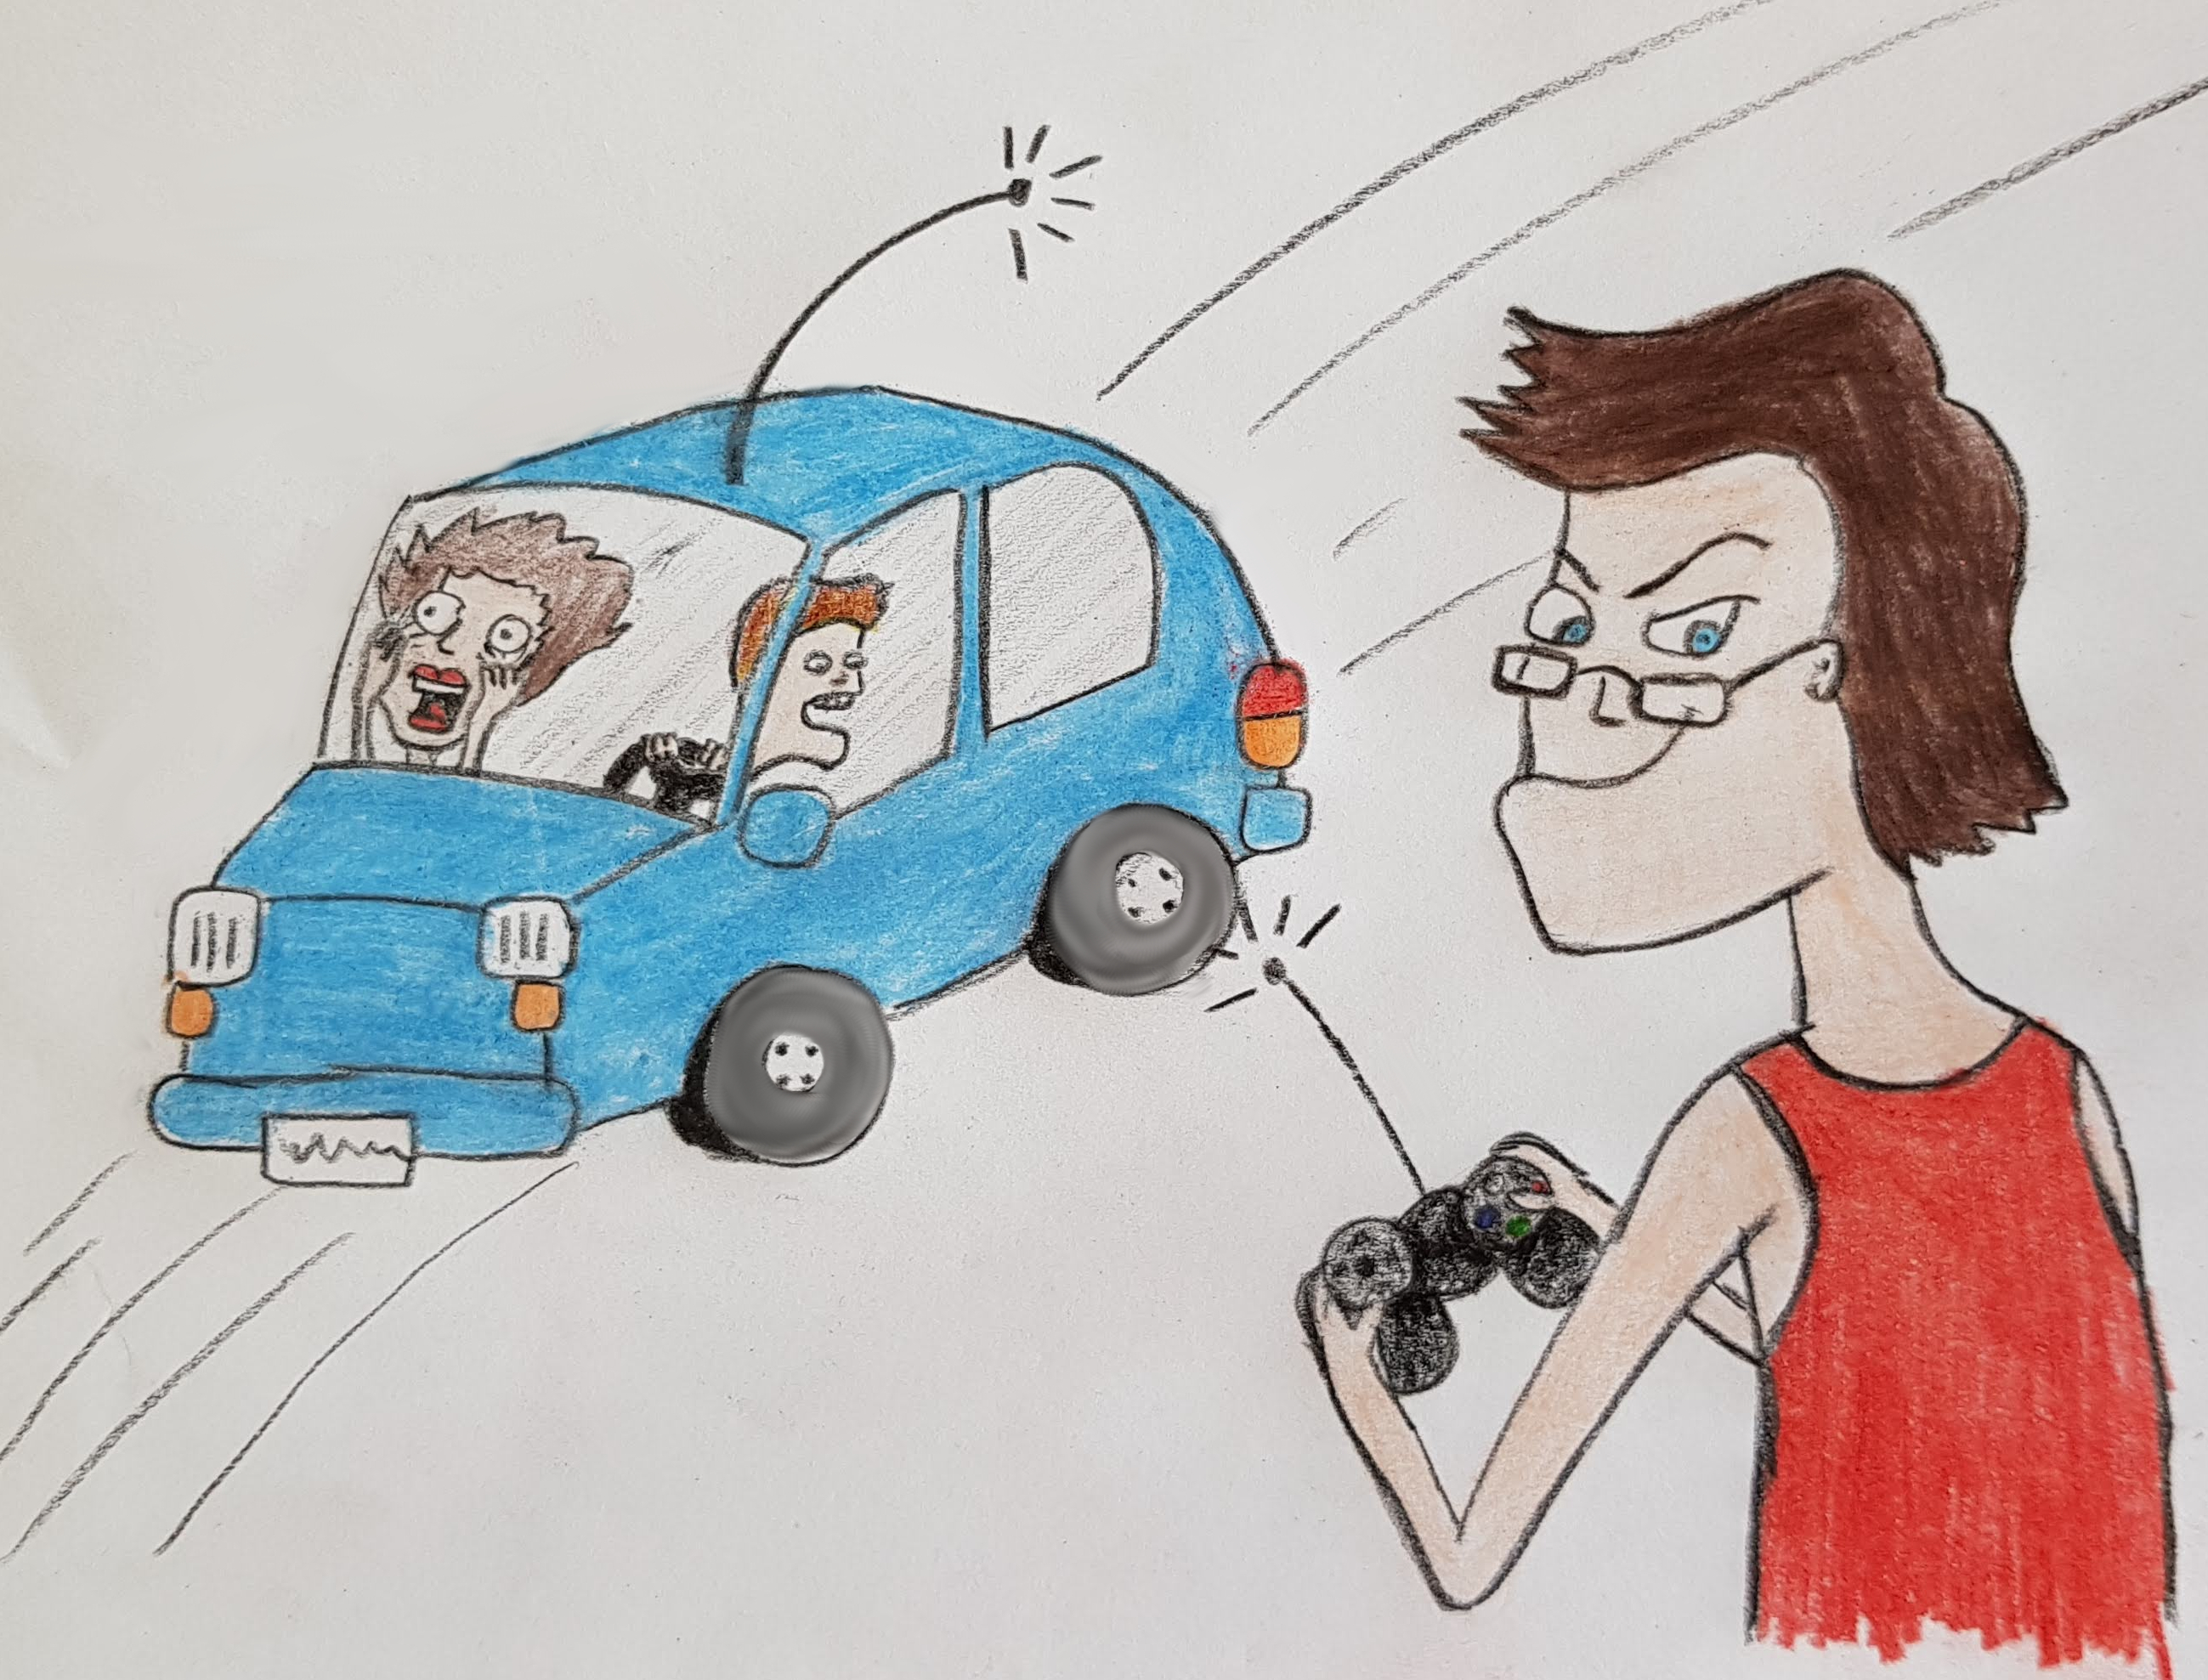
\includegraphics[width=1\linewidth]{Auto.jpg}
\end{figure}
\end{frame}

%------------------------------------------------

\begin{frame}
\begin{columns}[c]
\column{.65\textwidth}
\begin{itemize}
\item Kernel = Schlüsselkomponente für sichere Systeme
\item Zugriffsteuerung auf Hardwarekomponenten
\item Fehler im Kernel kann die Sicherheit und Verlässlichkeit des kompletten Systems zum erliegen bringen.
\item Monolithische Designs: 
\begin{itemize}
\item Große Menge Code
\item Integration weiterer Funktionen.
\item Folge: Grundlegend schwach durch größere Anfällgkeit für Bugs.
\end{itemize}
\end{itemize}
\column{.35\textwidth}
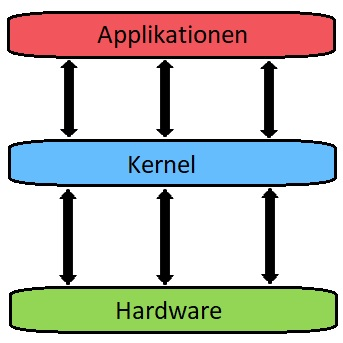
\includegraphics[width=0.8\linewidth]{Kernel.jpg}
\end{columns}
\begin{itemize}
\item Microkernel:\\
Konzentration auf die fundamentalen Funktionen eines Kernels: \\
z.B. Interprozesskommunikation, Scheduling, Speicherverwaltung
\item Durch Microkernels: Fehleranfälligkeit verringern (weniger Code $\Rightarrow$ Fehlerfreiheit formell verifizierbar)
\end{itemize}
\end{frame}

%------------------------------------------------
\section{seL4}
\begin{frame}
\frametitle{seL4}
\tikz[remember picture,overlay] 
   \node[anchor=north east,inner sep=0pt] 
    at([shift={(-1,-1.5)}]current page.north east){
\includegraphics[width=3cm]{sel4-logo.jpg}}; 
\begin{itemize}
\item In den 1990er Jahren entwickelt.
\item Basiert auf dem L4 Microkernel. 
\end{itemize}
\end{frame}
%------------------------------------------------
\begin{frame}
\begin{figure}[t]
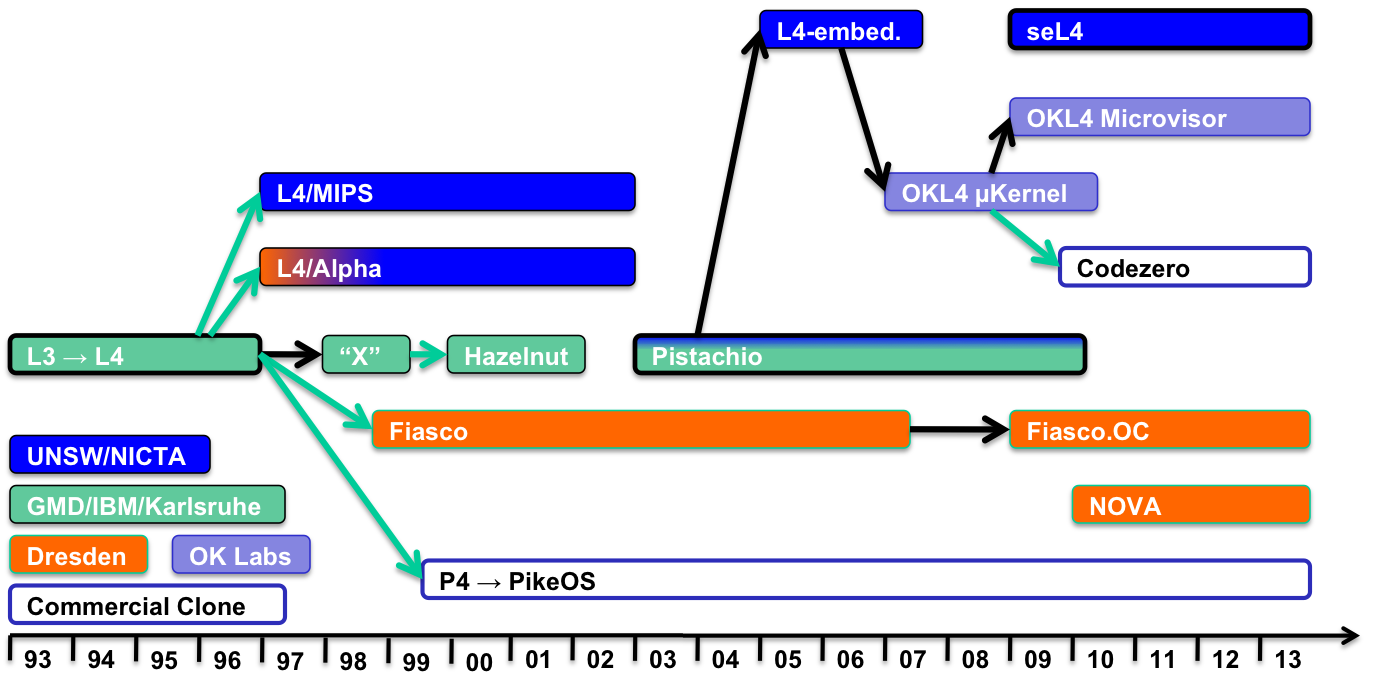
\includegraphics[width=1\linewidth]{L4tree.png}
\end{figure}
\end{frame}
%------------------------------------------------
\begin{frame}
\tikz[remember picture,overlay] 
   \node[anchor=north east,inner sep=0pt] 
    at([shift={(-1,-1.5)}]current page.north east){
\includegraphics[width=3cm]{sel4-logo.jpg}}; 
\begin{itemize}
\item In den 1990er Jahren entwickelt.
\item Basiert auf dem L4 Microkernel.
\item Stellt minimale Anzahl an services für Applikationen bereit. 
\end{itemize}
\end{frame}
%------------------------------------------------
\begin{frame}
\tikz[remember picture,overlay] 
   \node[anchor=north,inner sep=0pt]
    at([shift={(0,-1.5)}]current page.north) 		{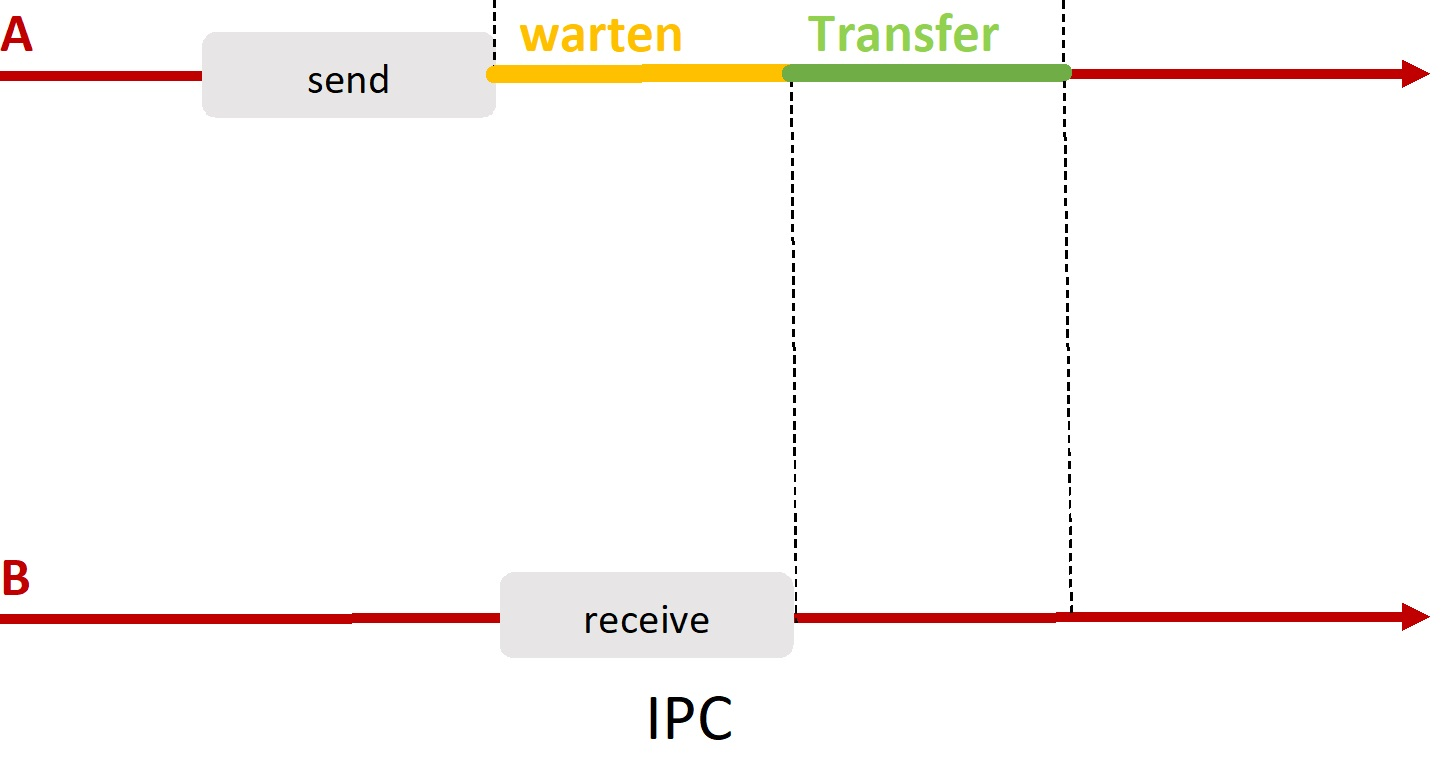
\includegraphics[width=5cm]{IPC2.jpg}};
\end{frame}
%------------------------------------------------
\begin{frame}
\tikz[remember picture,overlay] 
   \node[anchor=north,inner sep=0pt]
    at([shift={(0,-1.5)}]current page.north) 		{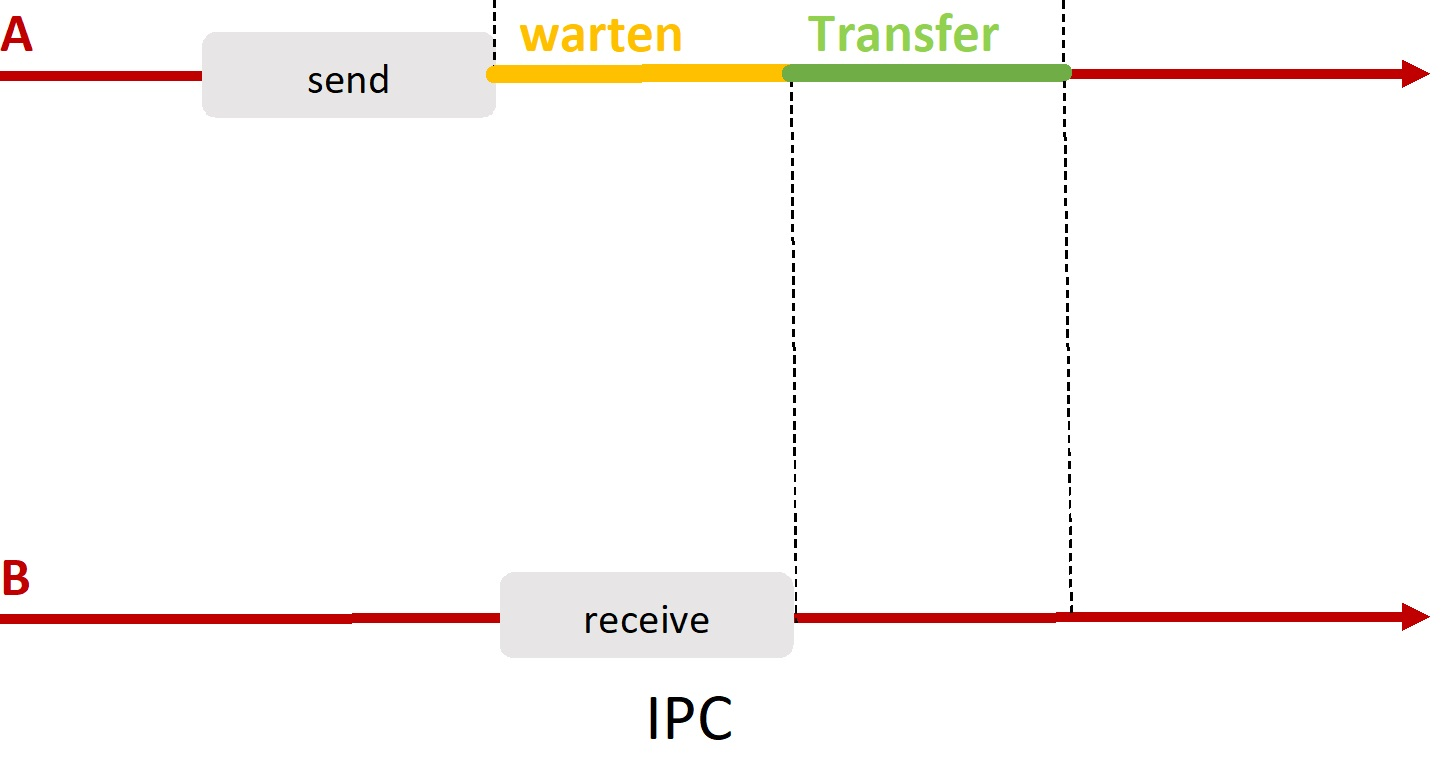
\includegraphics[width=5cm]{IPC2.jpg}};
\tikz[remember picture,overlay] 
   \node[anchor=south west,inner sep=0pt]
    at([shift={(2,1)}]current page.south west) 		{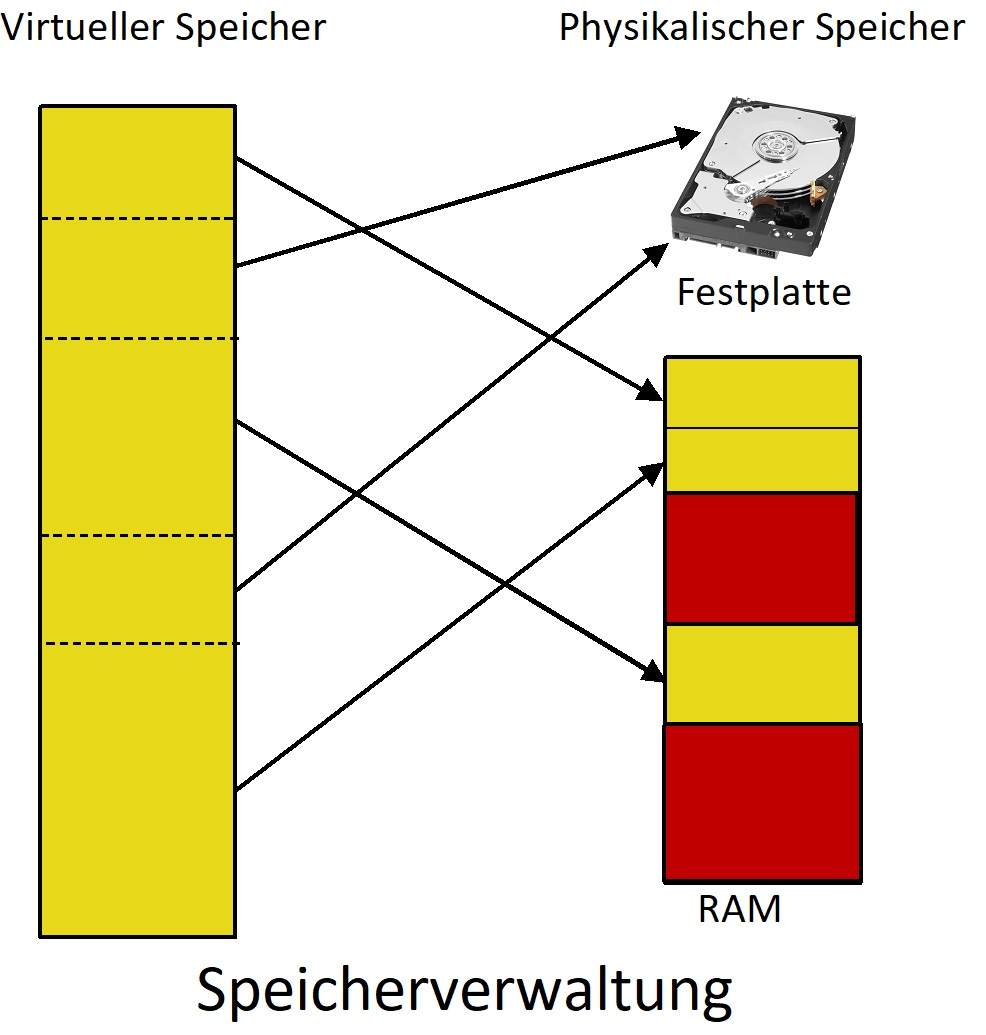
\includegraphics[width=4cm]{Speicher.jpg}};
\end{frame}
%------------------------------------------------
\begin{frame}
\tikz[remember picture,overlay] 
   \node[anchor=north,inner sep=0pt]
    at([shift={(0,-1.5)}]current page.north) 		{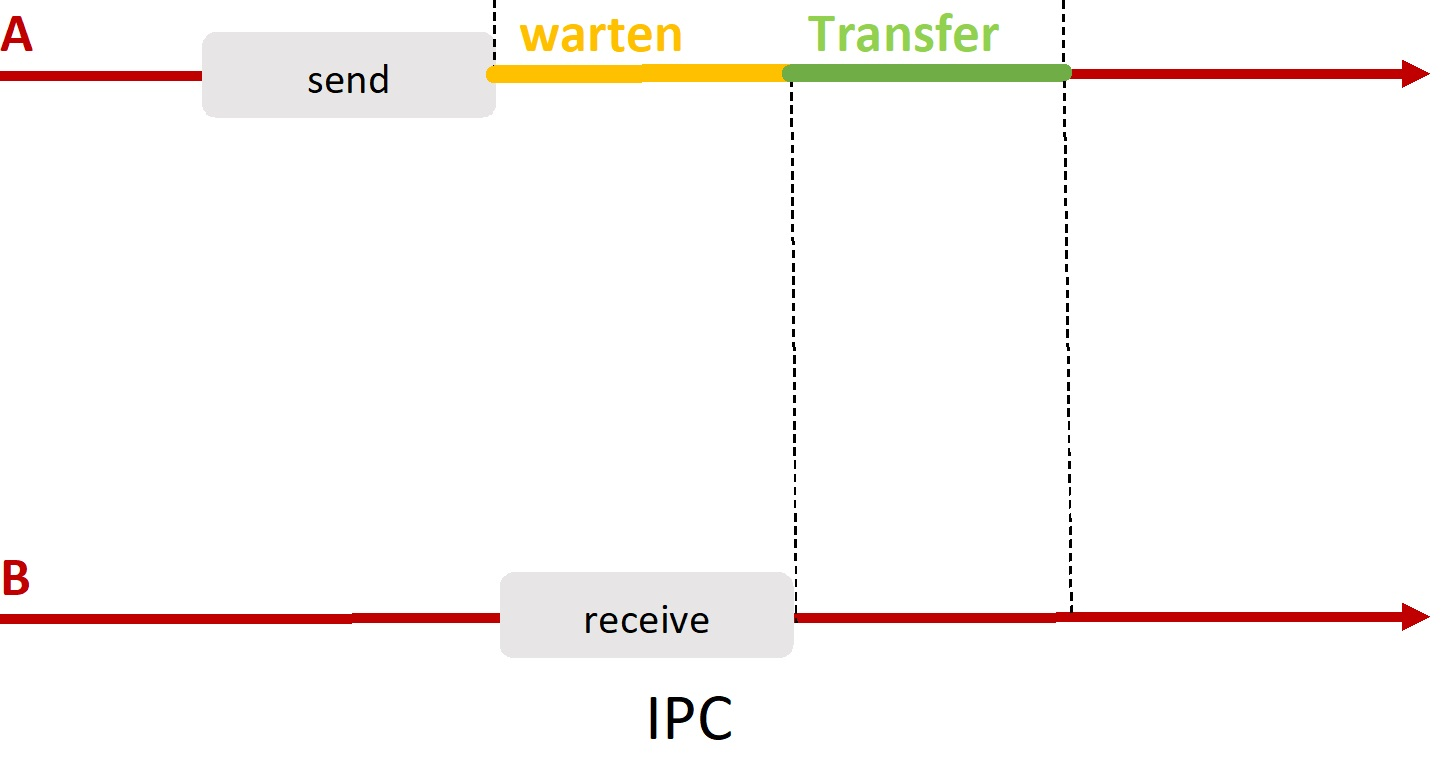
\includegraphics[width=5cm]{IPC2.jpg}};
\tikz[remember picture,overlay] 
   \node[anchor=south west,inner sep=0pt]
    at([shift={(2,1)}]current page.south west) 		{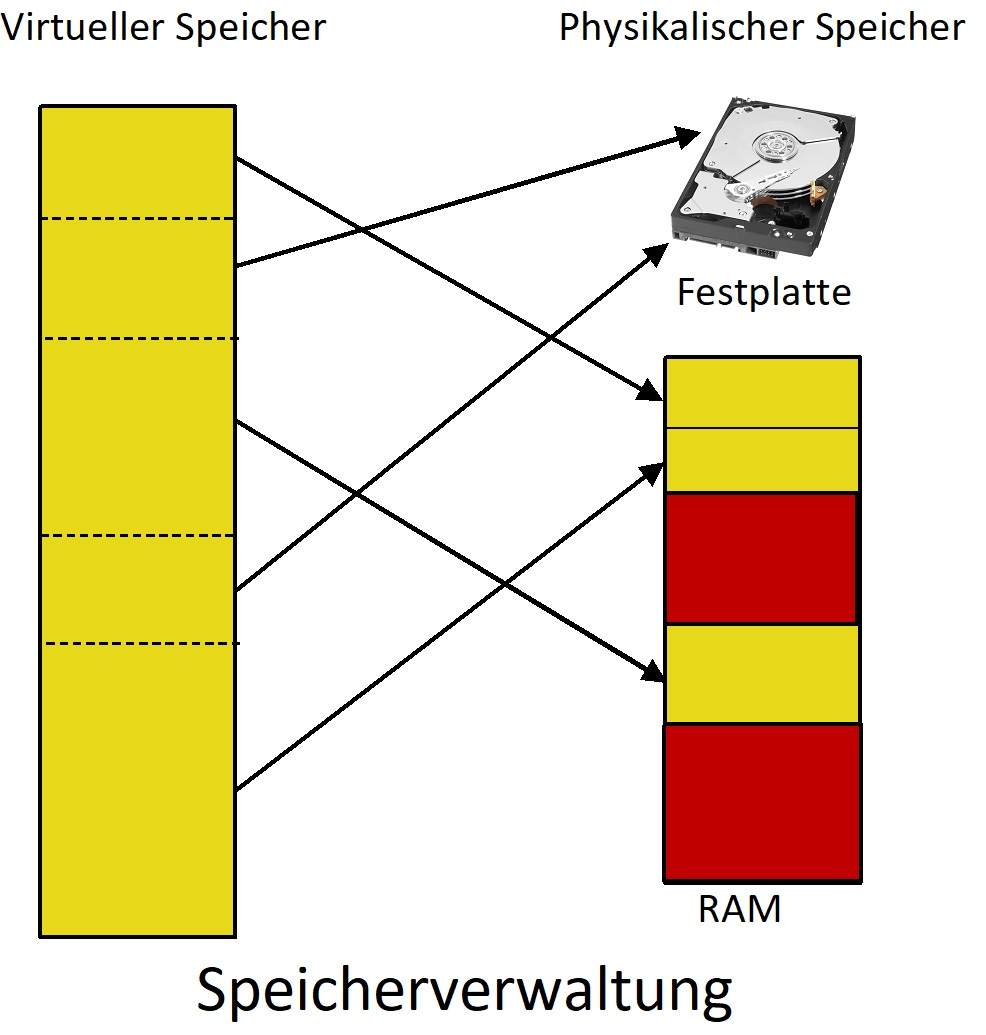
\includegraphics[width=4cm]{Speicher.jpg}};
    \tikz[remember picture,overlay] 
   \node[anchor=south east,inner sep=0pt]
    at([shift={(-2,1)}]current page.south east) 		{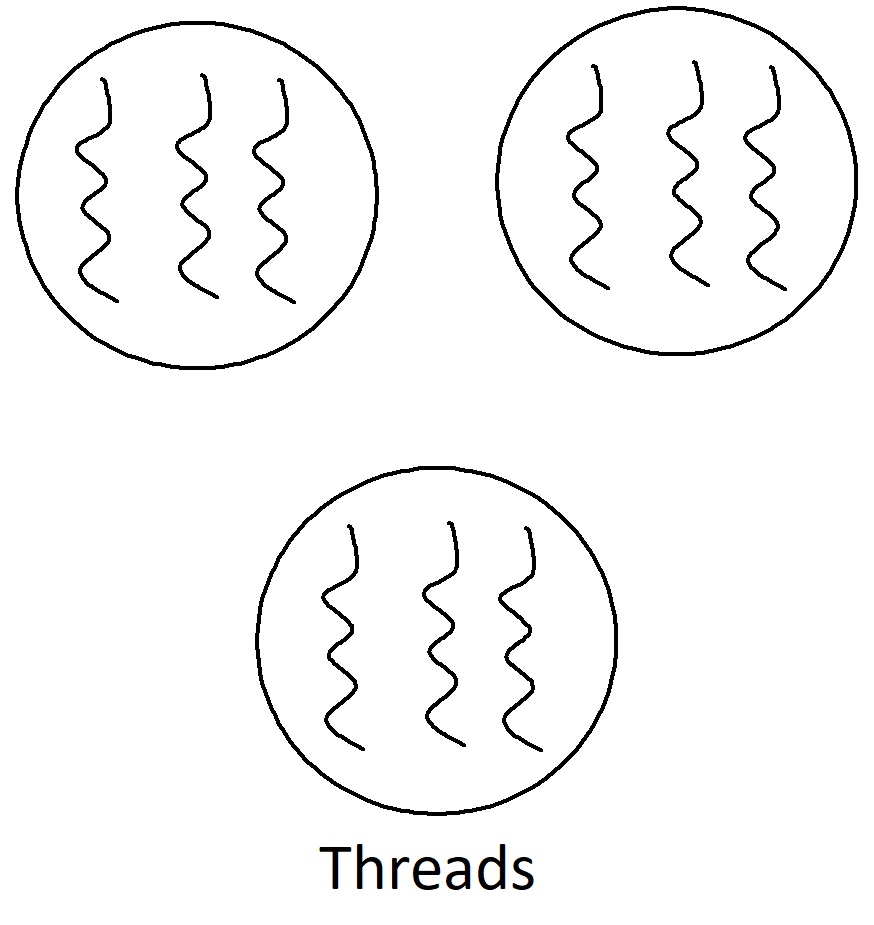
\includegraphics[width=3.5cm]{Threads.jpg}};
\end{frame}
%------------------------------------------------
\begin{frame}
\tikz[remember picture,overlay] 
   \node[anchor=north east,inner sep=0pt] 
    at([shift={(-1,-1.5)}]current page.north east){
\includegraphics[width=3cm]{sel4-logo.jpg}}; 
\begin{itemize}
\item In den 1990er Jahren entwickelt.
\item Basiert auf dem L4 Microkernel.
\item Stellt minimale Anzahl an services für Applikationen bereit. 
\item \textbf{Objekte:} implementieren jeweils die Abstraktion eines Services.
\end{itemize}
\end{frame}
%------------------------------------------------
\begin{frame}
\tikz[remember picture,overlay] 
   \node[anchor=north east,inner sep=0pt] 
    at([shift={(-1,-1.5)}]current page.north east){
\includegraphics[width=3cm]{sel4-logo.jpg}}; 
\begin{itemize}
\item In den 1990er Jahren entwickelt.
\item Basiert auf dem L4 Microkernel.
\item Stellt minimale Anzahl an services für Applikationen bereit. 
\item \textbf{Objekte:} implementieren jeweils die Abstraktion eines Services.
\item \textbf{Capabilities:} von Applikationen benötigt, um einen Service zu nutzen. 
\end{itemize}
\end{frame}
%------------------------------------------------
\begin{frame}
\tikz[remember picture,overlay] 
   \node[anchor=north east,inner sep=0pt] 
    at([shift={(-1,-1.5)}]current page.north east){
\includegraphics[width=3cm]{sel4-logo.jpg}}; 
\begin{itemize}
\item In den 1990er Jahren entwickelt.
\item Basiert auf dem L4 Microkernel.
\item Stellt minimale Anzahl an services für Applikationen bereit. 
\item \textbf{Objekte:} implementieren jeweils die Abstraktion eines Services.
\item \textbf{Capabilities:} von Applikationen benötigt, um einen Service zu nutzen. 
\item Die Rechte \texttt{Read, Write, Grant} und \texttt{Create} können in den Capabilities enthalten sein. 
\end{itemize}
\end{frame}
%------------------------------------------------
\begin{frame}
\begin{figure}[c]
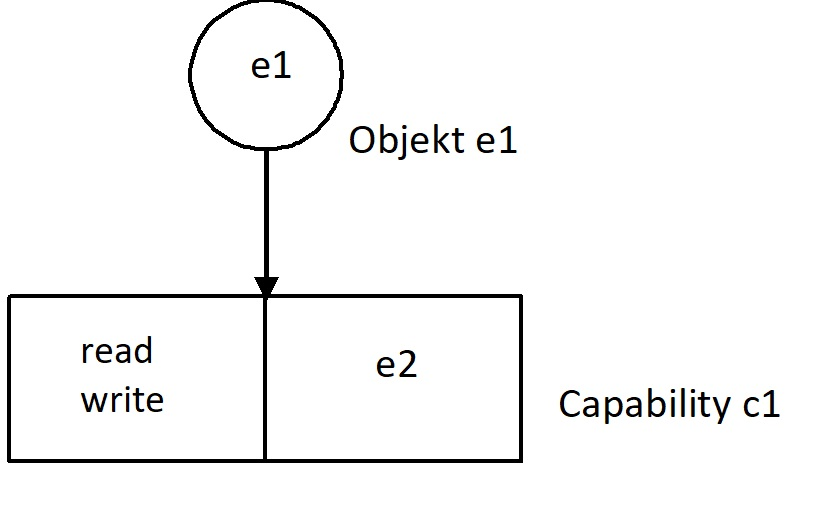
\includegraphics[width=4.5cm]{Capabilities1.jpg}
\end{figure}
\end{frame}
%------------------------------------------------
\begin{frame}
\begin{figure}[c]
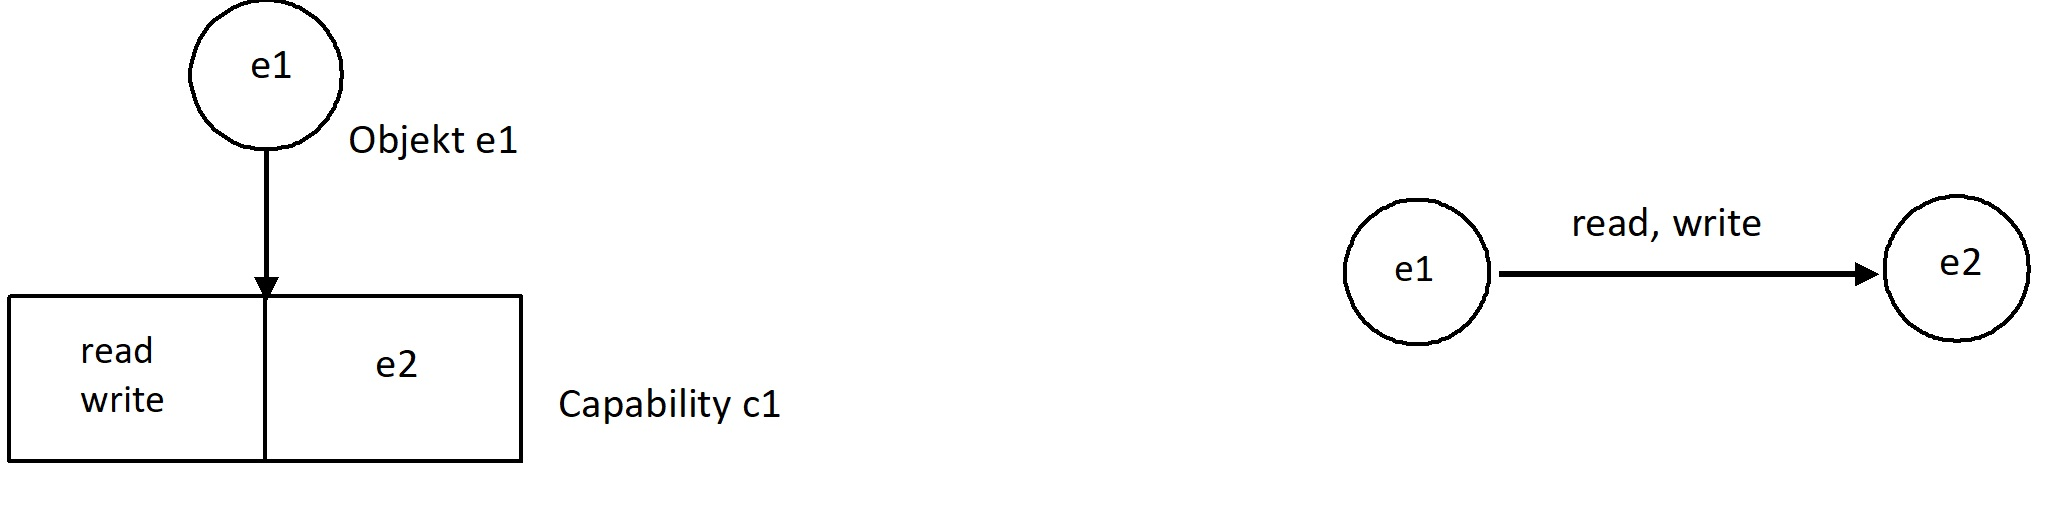
\includegraphics[width=10cm]{Capabilities2.jpg}
\end{figure}
\end{frame}
%------------------------------------------------
\begin{frame}
\subsection{Kernel Objekte}
\frametitle{Kernel Objekte}
\begin{itemize}
\item CNodes
\item IPC Endpoints
\item TCP
\item Virtual Memory
\item Interrupt Objects
\item Untyped Memory
\end{itemize}
\end{frame}
%------------------------------------------------
\begin{frame}
\frametitle{CNodes}
\begin{columns}[c]
\column{.65\textwidth}
\begin{itemize}
\item Lagern die Capabilities
\item Erhalten feste Zahl an Slots
\item Kernel konstruiert einen CDT (Capability Derivation Tree) zur Dokumentation der erstellten Capabilities und ihrer Verbindungen.
\end{itemize}
\column{.35\textwidth}
{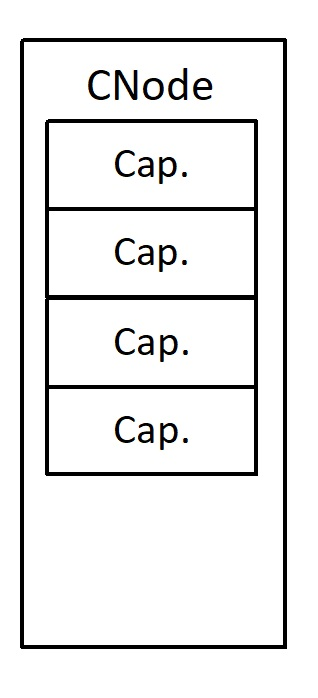
\includegraphics[width=1.5cm]{CNode.jpg}} \\~~
{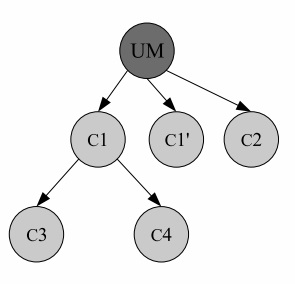
\includegraphics[width=2cm]{CDT.jpg}}
\end{columns} 
\end{frame}
%------------------------------------------------
\begin{frame}
\frametitle{Blocks of Highlighted Text}
\begin{block}{Block 1}
Lorem ipsum dolor sit amet, consectetur adipiscing elit. Integer lectus nisl, ultricies in feugiat rutrum, porttitor sit amet augue. Aliquam ut tortor mauris. Sed volutpat ante purus, quis accumsan dolor.
\end{block}

\begin{block}{Block 2}
Pellentesque sed tellus purus. Class aptent taciti sociosqu ad litora torquent per conubia nostra, per inceptos himenaeos. Vestibulum quis magna at risus dictum tempor eu vitae velit.
\end{block}

\begin{block}{Block 3}
Suspendisse tincidunt sagittis gravida. Curabitur condimentum, enim sed venenatis rutrum, ipsum neque consectetur orci, sed blandit justo nisi ac lacus.
\end{block}
\end{frame}

%------------------------------------------------

\begin{frame}
\frametitle{Multiple Columns}
\begin{columns}[c] % The "c" option specifies centered vertical alignment while the "t" option is used for top vertical alignment

\column{.45\textwidth} % Left column and width
\textbf{Heading}
\begin{enumerate}
\item Statement
\item Explanation
\item Example
\end{enumerate}

\column{.5\textwidth} % Right column and width
Lorem ipsum dolor sit amet, consectetur adipiscing elit. Integer lectus nisl, ultricies in feugiat rutrum, porttitor sit amet augue. Aliquam ut tortor mauris. Sed volutpat ante purus, quis accumsan dolor.

\end{columns}
\end{frame}

%------------------------------------------------
\section{Second Section}
%------------------------------------------------

\begin{frame}
\frametitle{Table}
\begin{table}
\begin{tabular}{l l l}
\toprule
\textbf{Treatments} & \textbf{Response 1} & \textbf{Response 2}\\
\midrule
Treatment 1 & 0.0003262 & 0.562 \\
Treatment 2 & 0.0015681 & 0.910 \\
Treatment 3 & 0.0009271 & 0.296 \\
\bottomrule
\end{tabular}
\caption{Table caption}
\end{table}
\end{frame}

%------------------------------------------------

\begin{frame}
\frametitle{Theorem}
\begin{theorem}[Mass--energy equivalence]
$E = mc^2$
\end{theorem}
\end{frame}

%------------------------------------------------

\begin{frame}[fragile] % Need to use the fragile option when verbatim is used in the slide
\frametitle{Verbatim}
\begin{example}[Theorem Slide Code]
\begin{verbatim}
\begin{frame}
\frametitle{Theorem}
\begin{theorem}[Mass--energy equivalence]
$E = mc^2$
\end{theorem}
\end{frame}\end{verbatim}
\end{example}
\end{frame}

%------------------------------------------------

\begin{frame}
\frametitle{Figure}
Uncomment the code on this slide to include your own image from the same directory as the template .TeX file.
%\begin{figure}
%\includegraphics[width=0.8\linewidth]{test}
%\end{figure}
\end{frame}

%------------------------------------------------

\begin{frame}[fragile] % Need to use the fragile option when verbatim is used in the slide
\frametitle{Citation}
An example of the \verb|\cite| command to cite within the presentation:\\~

This statement requires citation \cite{p1}.
\end{frame}

%------------------------------------------------

\begin{frame}
\frametitle{References}
\footnotesize{
\begin{thebibliography}{99} % Beamer does not support BibTeX so references must be inserted manually as below
\bibitem[Smith, 2012]{p1} John Smith (2012)
\newblock Title of the publication
\newblock \emph{Journal Name} 12(3), 45 -- 678.
\end{thebibliography}
}
\end{frame}

%------------------------------------------------

\begin{frame}
\Huge{\centerline{The End}}
\end{frame}

%----------------------------------------------------------------------------------------

\end{document} 
